\documentclass[conference]{IEEEtran}
\usepackage{cite}
\usepackage{amsmath,amssymb,amsfonts}
\usepackage{algorithmic}
\usepackage{graphicx}
\usepackage{textcomp}
\usepackage{xcolor}
\def\BibTeX{{\rm B\kern-.05em{\sc i\kern-.025em b}\kern-.08em
    T\kern-.1667em\lower.7ex\hbox{E}\kern-.125emX}}
    
\usepackage{float}
\usepackage[caption=false]{subfig}
\usepackage{url,hyperref}
\usepackage{multirow}

\begin{document}

\title{MoReL: Molecule Representation Learning Toolkit\\
	{
		\footnotesize \textsuperscript{}
	}
		\thanks{}
}

\author{
	\IEEEauthorblockN{
		Songhao Jiang\IEEEauthorrefmark{1}, 
		Xiaotian Duan\IEEEauthorrefmark{2},
	}
	\IEEEauthorblockA{
		\textit{Department of Computer Science} \\
		\textit{The University of Chicago}\\
		Emails: \IEEEauthorrefmark{1}shjiang@uchicago.edu, \IEEEauthorrefmark{2}xduan7@uchicago.edu,
	}
}

\maketitle

\begin{abstract}
There are multiple ways to featurize molecules, and more than a couple of suitable deep learning models for any one of these features. 
Moreover, for each one of the combinations between features and models, there are different sets of hyper-parameters, like learning rate, dropout rate, etc., to explore. 
The combinatorial number of learning instances to run is in the scale of thousands if not more, which makes it crucial to have a robust and efficient system to help us with data loading, as well as the arrangement and parallelization of the jobs. 

In this paper, we propose a system, MoReL, that can take advantage of the data parallelism during hyper-parameter searching, and accelerate the whole training process.
\end{abstract}

\begin{IEEEkeywords}
deep learning, system, molecule, representation learning
\end{IEEEkeywords}

\section{Introduction} \label{sec_intro} 

The properties of a molecule is at the heart of many problems, from drug synthesis to material discovery. 
With the rising popularity of deep learning and the support of underlying hardwares, more and more efforts have been put into the research of representation learning of molecules using neural networks. 
However, unlike images or natural language corpora, featurizing (transforming into vectors of numbers for statistical learning) molecules is rather unintuitive. 
Thus, different ways of featurization have been invented to incorporate human understanding of the molecules into learning models, like SMILES (Simplified molecular-input line-entry system) strings, fingerprints \cite{ecfp}, descriptors, and graphs. 

Each of these distinct molecular features is suitable for a different set of deep learning models. 
For example, SMILES strings (e.g. "(C=O)=O", "C1CCCCC1"), which are entirely made of ASCII characters, are preferably trained on NLP (natural language processing) models like LSTM \cite{lstm} or Transformer \cite{transformer}. 
Similarly, molecular graph features are usually fed into neural networks that are designed for learning graphs, like GGNN \cite{ggnn} or GCN \cite{gcn}. 

Moreover, for each combination of features and models, we need to experiment with different hyper-parameters, like dropout rates and optimizer configurations, in order to get better performance. 
A model might behave badly or even unstable using one set of hyper-parameters but beat records using another set. 

To sum things up, there are three main components in this projects from machine learning point of view: featurizers, models, and hyper-parameter searching. 
An overall flowchart of featurizers and models in this project is shown in Figure \ref{fig:train}, which highlights the relations between all different kinds of features and models planned in this project. 
The goal is to learn a meaningful and unique representation of molecules, by searching through all possible featurization methods, models, and hyper-parameters, which leads to the motivation of MoReL: to build a efficient light-weight system that enables the comparison between thousands of instances for molecular representation learning.

While the structure of the training and searching process looks straight-forward, the combinatorial number of learning instances is at least in the scale of thousands. 
Other than the number of instances that we need to run, there are a few challenges for this project:
\begin{itemize}
	\item[$\bullet$]  There are about 97 million molecules to train with, which take up to 10TB after featurization. With such scale, dataloading can easily become the bottleneck for training;
	\item[$\bullet$]  More about dataloading: the system is meant to be deployed on a supercomputer made up with a lot of CPUs, which means that the traditional approach (data prefetching with CPU and training with GPU at the same time) is no longer available. CPUs will be responsible of both dataloading and training, which means that the efficiency of dataloading is especially important in this project;
	\item[$\bullet$]  Some learning methods already have their Python scripts. We would like our toolkit to utilize the existing code with minimal changes. This will not only save a lot work, but also enable MoReL to be used on other projects that requires hyper-parameter optimization with existing training scripts. 
\end{itemize}

The layout of this paper is as follows: 
section \ref{sec_rw} talks about some previous works that are similar or related to ours; 
section \ref{sec_impl} contains different versions of implementations and details; 
section \ref{sec_eval} includes the evaluations of the aforementioned implementations. 

\begin{figure*}[!htb] 
	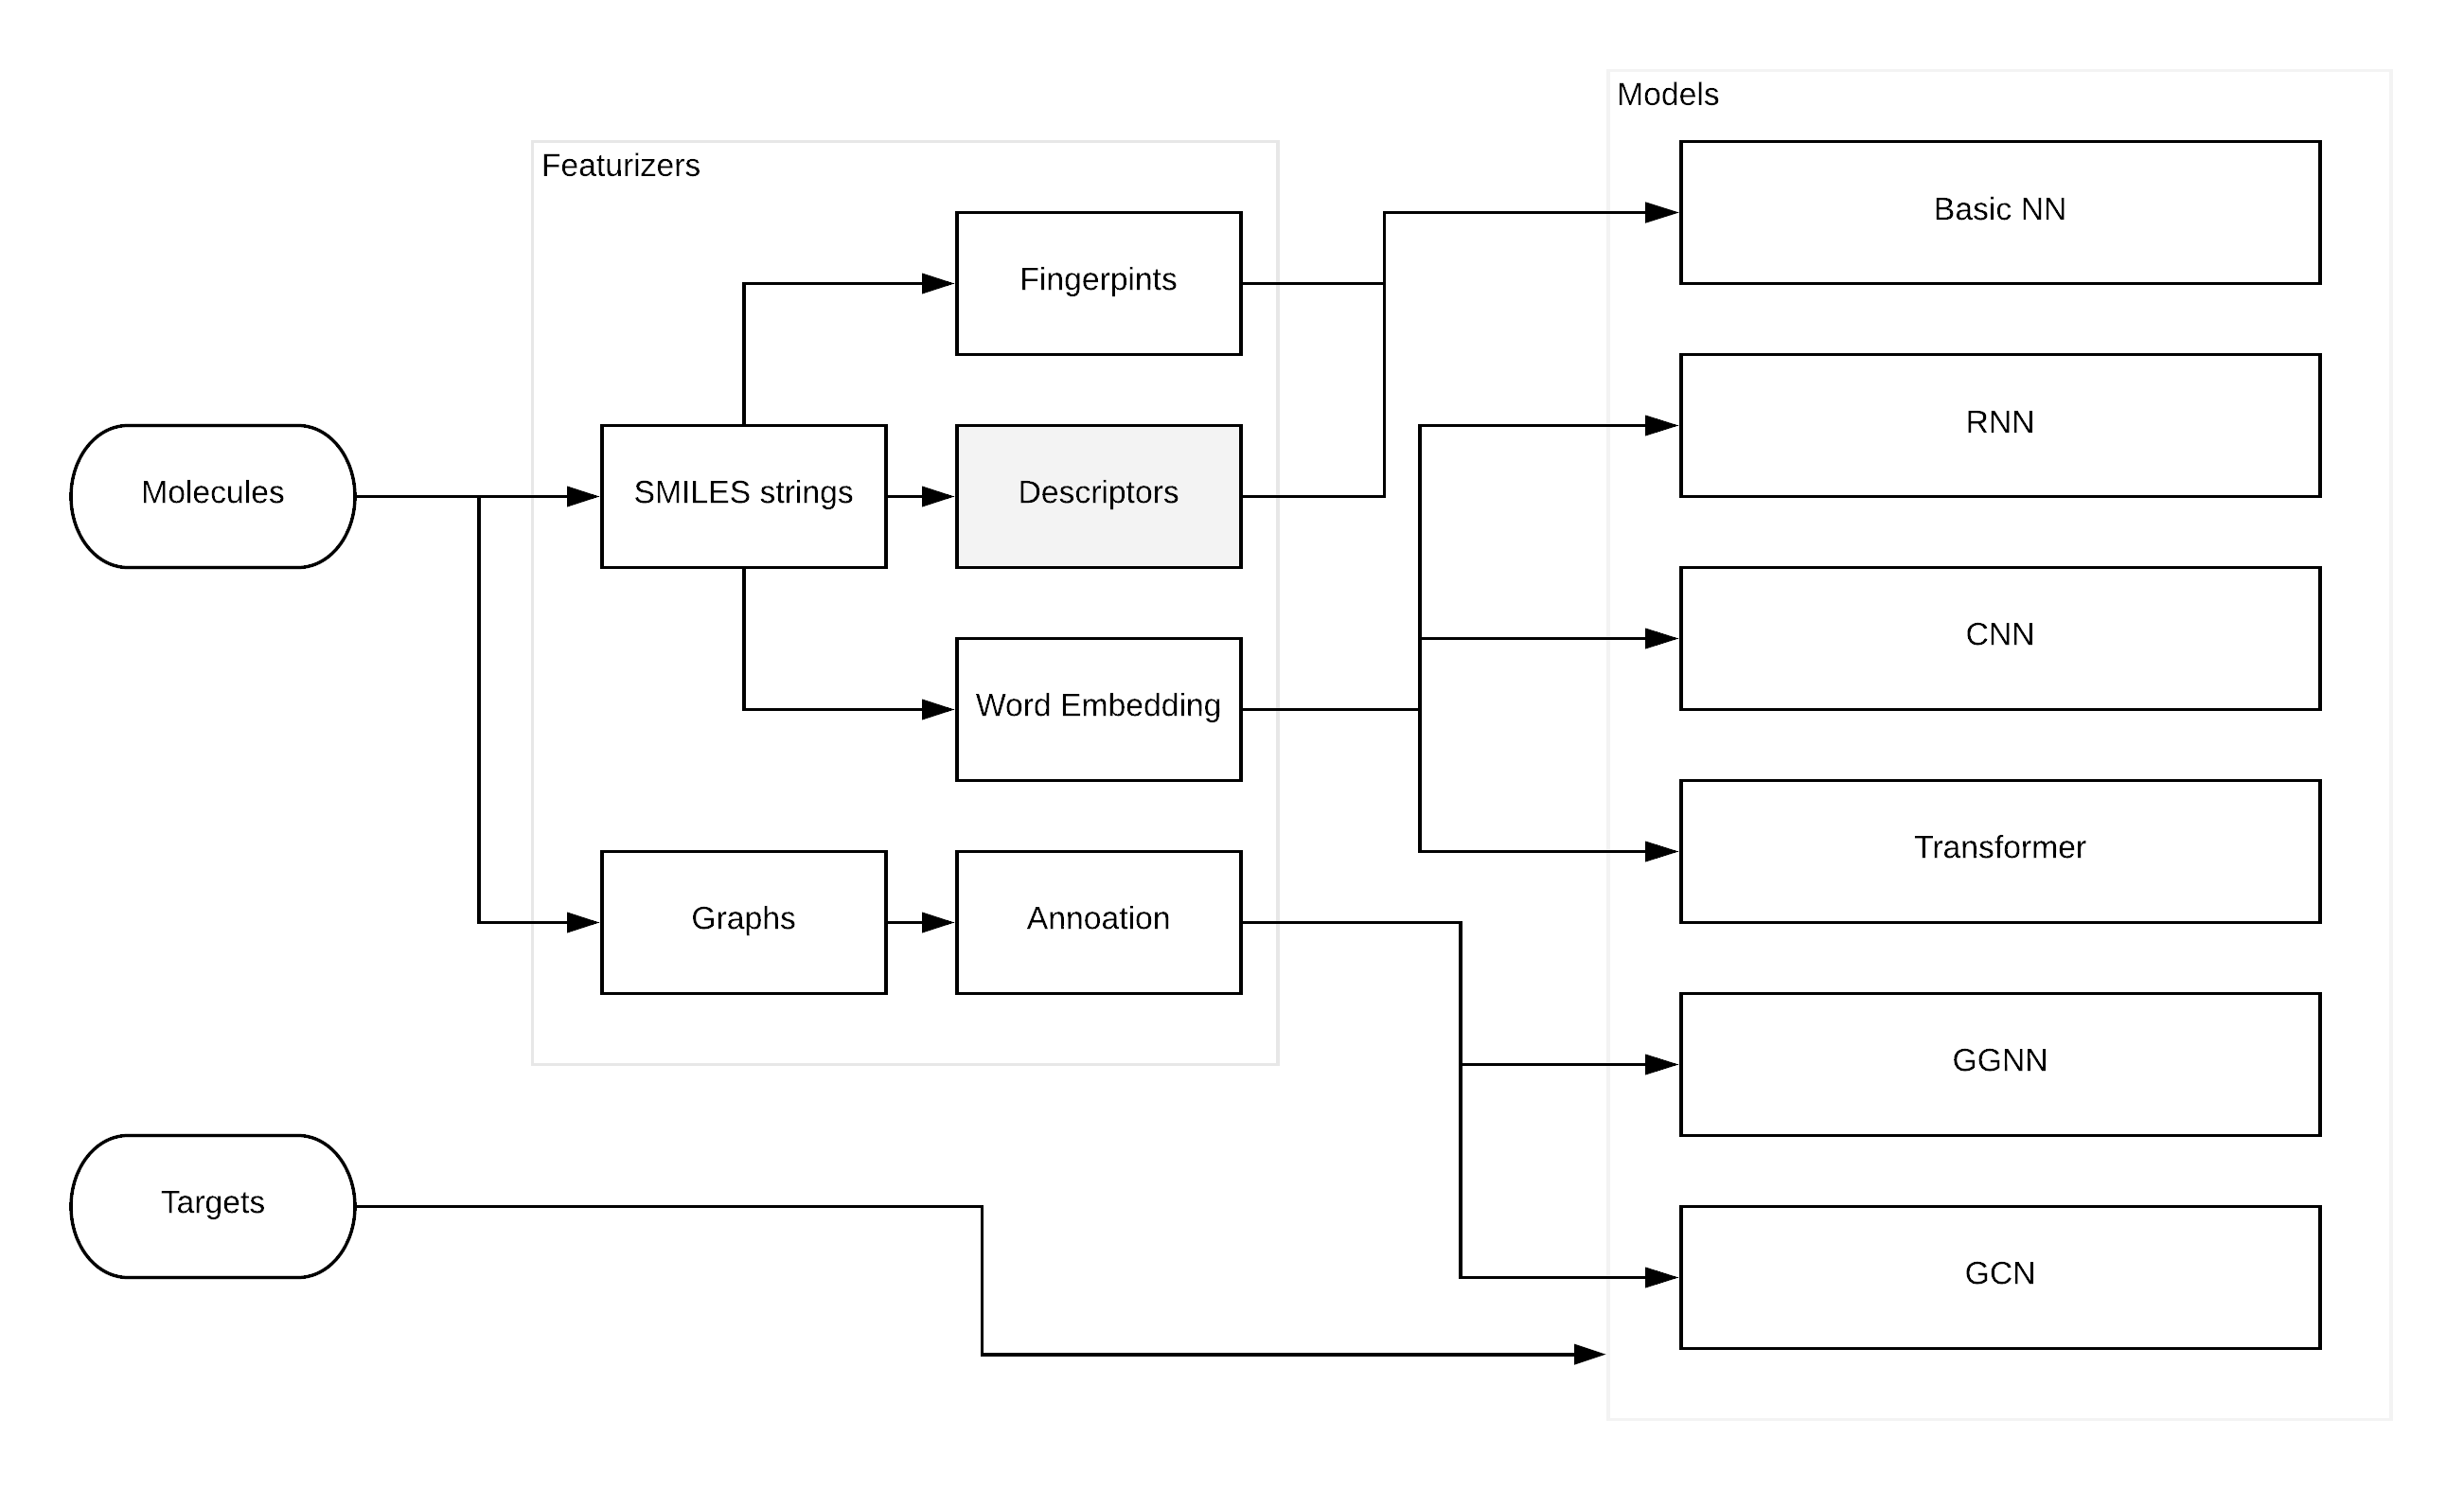
\includegraphics[width=\linewidth]{train.png}
	\caption{\small Training process flowchart. }
	\label{fig:train}
\end{figure*}

\section{Related Work} \label{sec_rw}

Significant works have been done for the comparison between different methods for molecule representation learning. 
For example, \cite{gagcn} has compared the performances with GGNN, GCN, and some variations on molecular learning; \cite{smiles2vec}, \cite{chemception} have tried using SMILES strings and molecular images as features, and tested with some generic models on benchmark datasets. 
However, the comparisons in these works are usually not comprehensive enough to cover a full spectrum of different featurization methods or network structures. 

More similar to our project, MoleculeNet \cite{molnet} is a framework that provides all necessary tools and an environment for comparing a variety of features (fingerprints, graphs, etc.) using different learning algorithms including deep learning, by evaluating performances on benchmark datasets (HIV, MUV, etc.). 
It serves to offer a ready-to-launch benchmark that users can evaluate their models back to back against existing ones. 
Our work differs from MoleculeNet in the following aspects:
\begin{itemize}
	\item[$\bullet$]  MoReL focuses only on deep learning models, with huge amount of training data (around 90 million). MoleculeNet is more inclusive in terms of learning algorithms, but only trains on benchmark datasets in a much smaller scale (less than 500 thousand);
	\item[$\bullet$]  MoReL is designed to train multiple instances in parallel on multiple GPUs, and searches for the best combination of features, model, and hyper-parameters. MoleculeNet has no such function;
	\item[$\bullet$]  The implementation of MoReL focuses on the efficiency, and can be easily applied to any deep learning project that requires hyper-parameter searching; 
\end{itemize}

\section{Implementation} \label{sec_impl} 

The basic idea behind this project is simple: during the hyper-parameter training, there will be a lot of models to train, and many of them are quite similar. 
If we can parallelize and synchronize models that use same features and have similar training speed, we can make them share the batches of features with each other. 
By doing so, we can reduce the number of data retrieval, and hence make the overall training process more efficient. 
Figure \ref{fig:dl} demonstrates such data sharing: by switching from \hyperref[dl_a]{(a)} to \hyperref[dl_b]{(b)}, we can save a huge amount of time spent on excessive dataloading.

\begin{figure}[!htb] 
	\subfloat[Naive implementation of data loading]{%
	  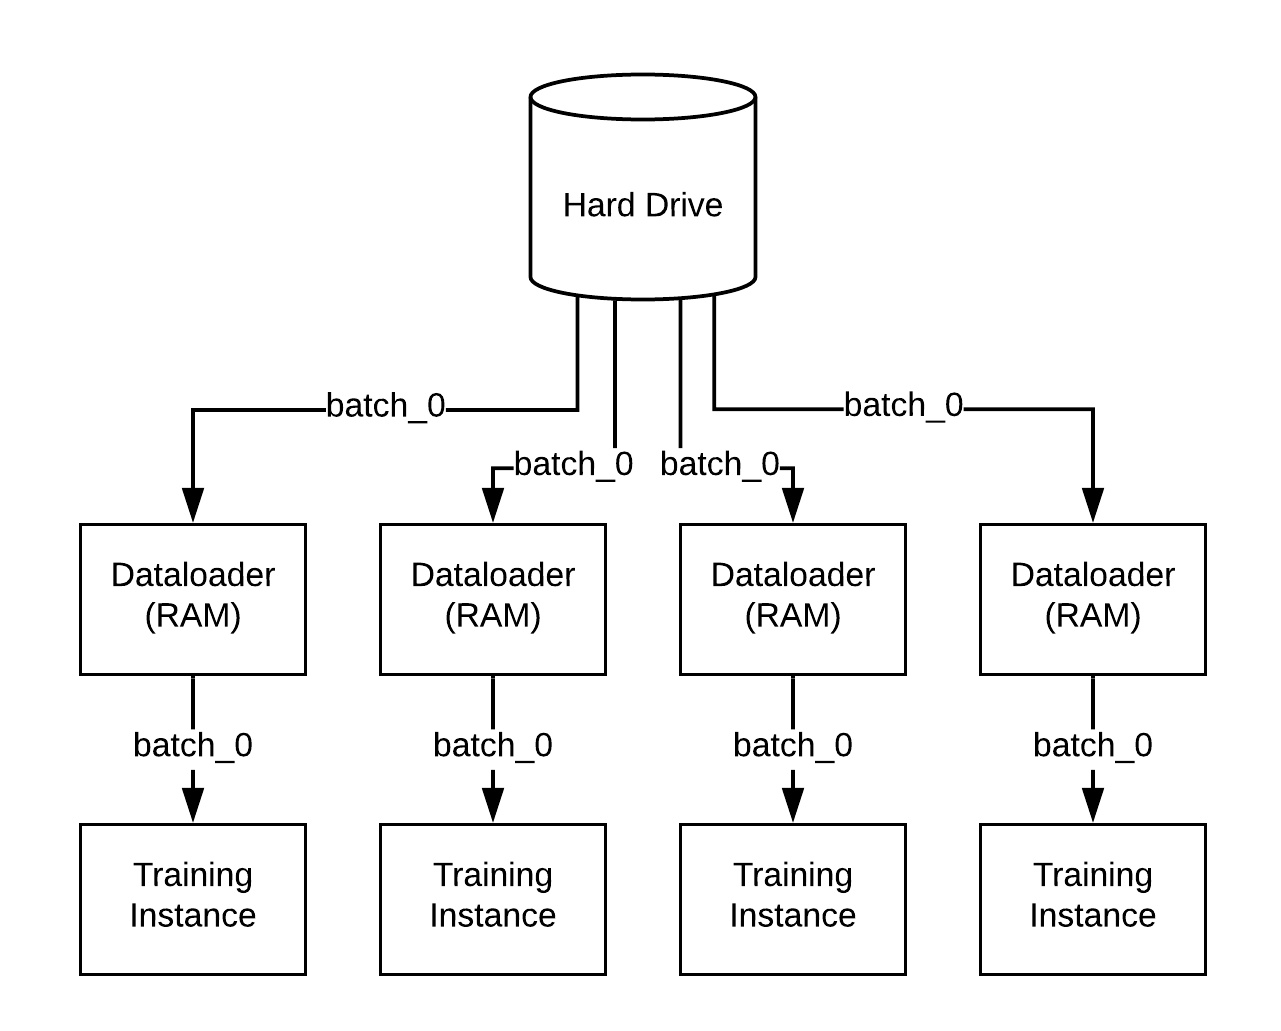
\includegraphics[width=.9\linewidth]{dataloading_a.png} 
	  \label{dl_a} 
	}
	
	\subfloat[Shared data loading]{%
	  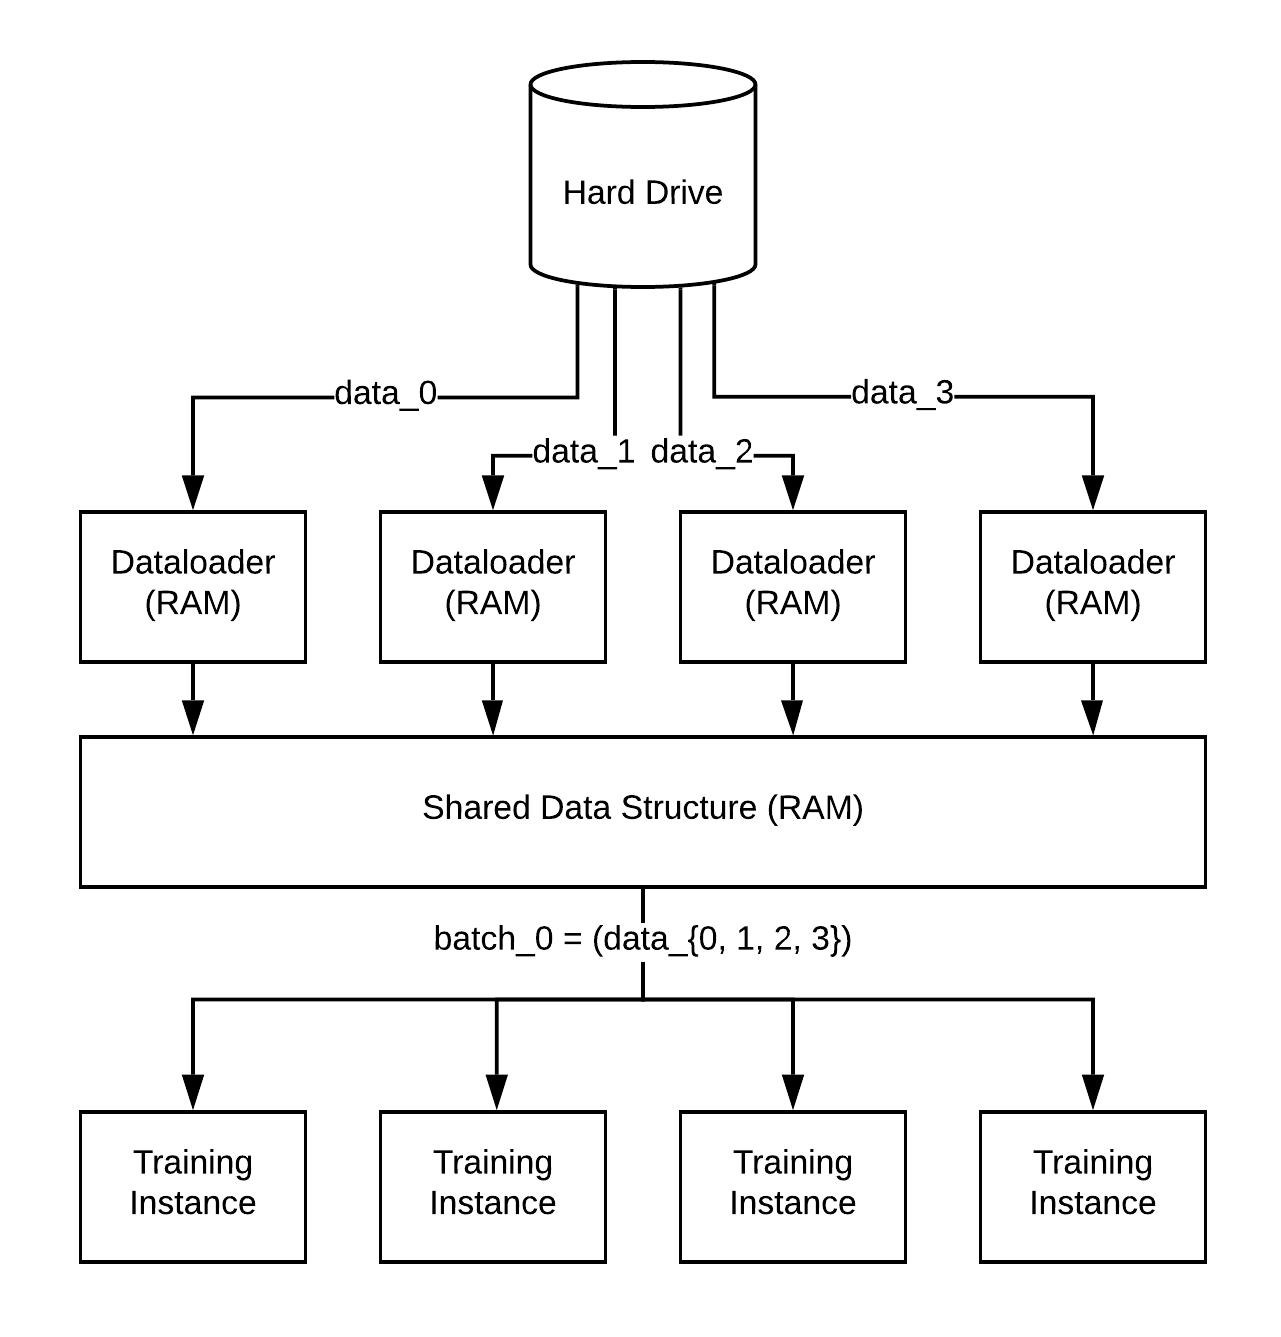
\includegraphics[width=.9\linewidth]{dataloading_b.png} 
	  \label{dl_b} 
	}
	
	\caption{\small 
		Original approach \hyperref[dl_a]{(a)} has excessive amount of data retrieval, reducing the efficiency of training process; 
		in \hyperref[dl_b]{(b)}, all the training instances are parallelized and synchronized so that they are using the exact same feature at the same time, and all the dataloaders from different learning instances are cooperating on data retrieval. }
	\label{fig:dl}
\end{figure}

In the following sections, we are going over the implementation details. 
Specifically, in \ref{subsec_dr}, we are going to discuss the design choices that we made for more efficient data retrieval; then we will cover the data sharing across Python processes in \ref{subsec_ds}; while \ref{subsec_oi} is about the original implementation that turned out to be sub-optimal; finally in \ref{subsec_ci}, the actual implementation that helps boosting the performance of the dataloading by a significant margin.

\subsection{Data Retrieval} \label{subsec_dr} 

For the input data in this project, we are using molecular InChI(The IUPAC International Chemical Identifier) from PubChem, which is directly accessible from PubChem FTP server. 
To extract the training features, RDKit, an open-source cheminformatics software will be used to obtain SMILES strings, fingerprints, and graphs directly from InChI with ready-to-use APIs. 
There are some existing work on how to extract more relevant graph features from molecules like \cite{gcn_fp}. In this project, we are using similar molecular graph features. 

However, now we are facing a simple but yet not obvious design choice: do we (1) pre-compute molecular features, store them in hard drives, and load them during training. or (2) compute the molecular features during training? 
During the project proposal and initial planning, we assumed that option (1) is faster because loading data from hard drive involves no computation and processing. 
However, the caveat of option (1) is that, we don't have enough space in SSD to hold all 10TB of pre-computed features, which means that option (1) implies loading data from HDD, while option (2) can utilize SSD as unfeaturized molecules only take about 50GB. 

There are some pros and cons for both options. 
For example, the biggest advantage for option (1) is that, the feature sharing turns out to be extremely easy: when one dataloader loads the features from hard drive, the operating system will cache the data in memory automatically, which means that all the other dataloaders can share the same features for a short amount of time. 
As long as we make sure that all training instances are synchronized, the data sharing is almost always enabled without any extra effort. 
Another big advantage for option (1) is that, pre-computed features are reusable not only for this project, but also for further experiments and researches. 
But on the other hand, option (2) is more flexible, which means that we can tweak the featurization methods on the fly, make changes to the features whenever and however we want. 

All these pros and cons are important, but ultimately we would like to pick the one with faster data retrieval speed. The performance comparison of data retrieval is shown in Figure \ref{fig:sp}. 
Note that we don't have enough SSD space to host all the pre-computed features, which means that "loading from HDF5 in SSD" is not really available. 
Computing features from molecules that are loaded from SSD is more than 10 times as fast as directly loading pre-computed features from HDD. 
If we are loading the whole dataset, which includes 97 millions of molecules, computing features could save us more than 15 days for processing time comparing to loading pre-computed features from HDD in a single training epoch. 

\begin{figure*}[!htb] 
	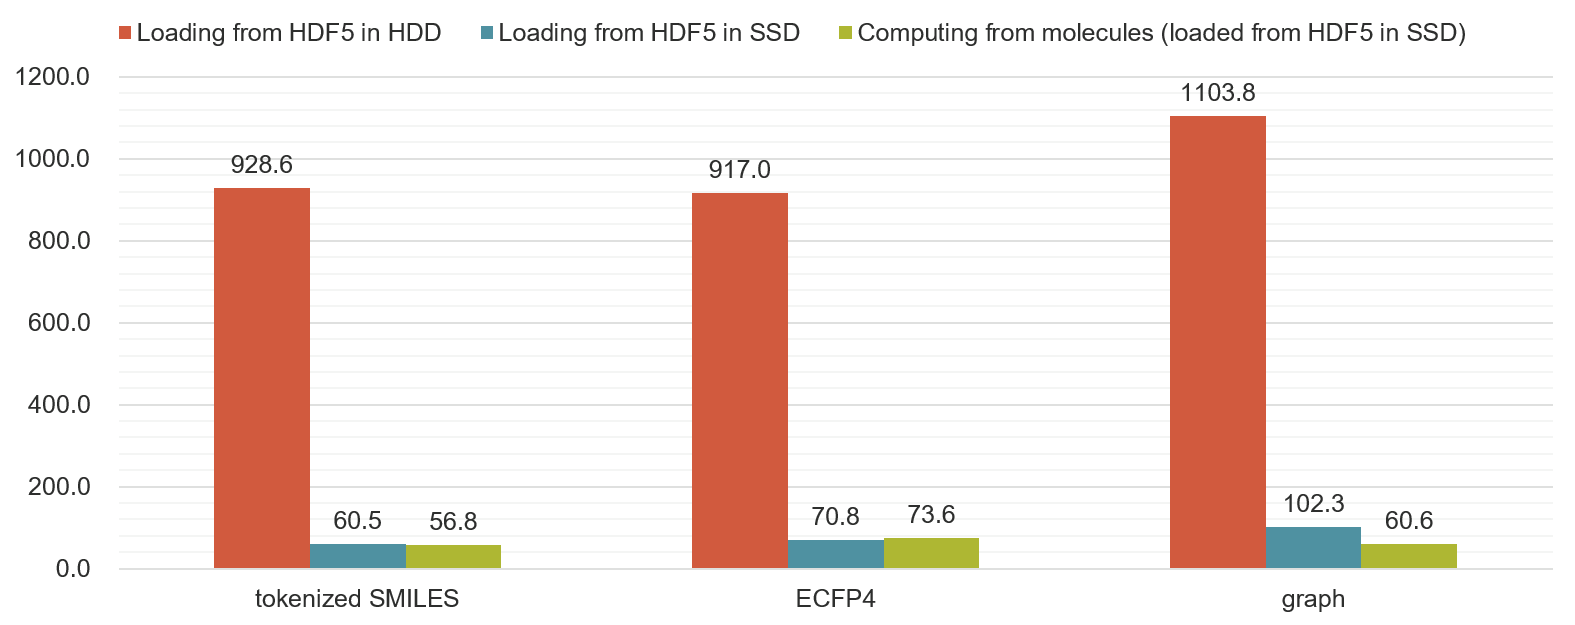
\includegraphics[width=\linewidth]{speed.png}
	\caption{\small Time in Seconds for Retrieving 65536 Features with Different Featurization Methods. }
	\label{fig:sp}
\end{figure*}

Apparently, for the sake of overall performance, we need to stick with computing features during training, which means that we need to take care of feature sharing explicitly. 
More specifically, we need to implement the shared data structure shown in Figure \ref{fig:dl}\hyperref[dl_b]{(b)} by ourselves, along with synchronization, garbage collection, and data region protection. 

\subsection{Data Sharing} \label{subsec_ds}

All training instances are independent Python processes. 
In order to share features among these instances, we need to consider how to explicitly maintain a data structure that are accessible to different processes.
Generally speaking, there are two different ways to share data across processes: (1) using shared memory, or (2) using a local server. 

For the first approach, we picked MMAP (memory-mapped files). 
Basically, we will allocate a chunk of memory, and share it between multiple processes as if it is a local file, and perform bytes read/write operations bytewise. 
The potential advantage of this approach is that, it directly interacts with memory and could be faster compared with other data sharing approaches. 
However, it comes with the price that we need to take care of the MMAP file in byte level. Every time we perform read and write, we have to translate the data unit into bytes, which could slow things down a little. 
Moreover, since it is a file that is shared among multiple processes, if there are situations where multiple processes are writing into the same file, we need to protect it with mutual exclusion in order to make sure of the data integrity. 

For the second approach, there is a  ready-to-use implementation in Python, named Manager (Proxy). 
The idea is to launch a server dedicated for a shared data structure. 
The clients (training instances) can perform read/write to the data just like it is local, without worrying about the data integrity. 
It is simple to implement but overhead introduced by network communication could be significant. 

In both approaches, we need to take care of the garbage collection: the data structure that holds the shared features need to be cleaned up every now and then.

In the following subsections about implementation, both data sharing methods are experimented and evaluated.


\subsection{Original Implementation} \label{subsec_oi}

The initial implementation is conceptually simple, but turns out to be sub-optimal in performance. 

The idea is to make garbage collection and featurization jobs as some kind of first-come-first-serve responsibility. 
Suppose that a training instance finishes the previous training batch before other training processes, it would first perform garbage collection to clean up the out-dated features in the shared data structure, and then starts featurizing molecules for the next batch, one molecule at a time.
Other training instances, once finished previous training batch, will join the featurization process. 
Consider the featurization of molecules as jobs in a pool, and each process/instance will act like independent workers that takes one molecule from the pool, performs computation, stores the feature in the shared data structure, and repeat if there are more jobs to do.
Soon we will have all the molecules in the next batch featurized. 
Finally, all the training instances will fetch the complete batch from shared data structure and continue training. 
An example of such parallelization is shown in the Figure \ref{fig:oi}. 

\begin{figure}[!htb]
	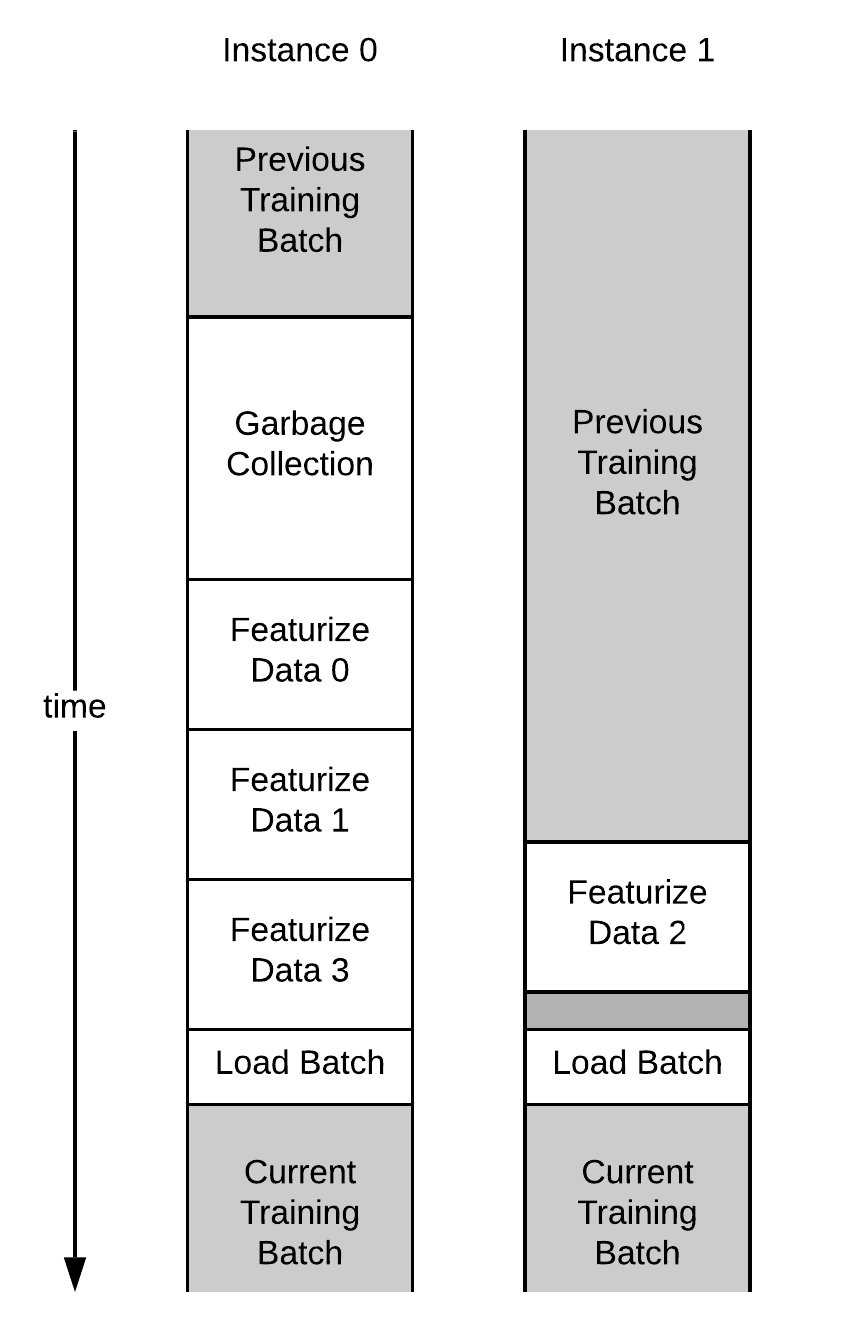
\includegraphics[width=\linewidth]{oi.png}
	\caption{\small 
		Featurization parallelization in the original implementation, with two training instances and batch size of 4. }
	\label{fig:oi}
\end{figure}

This implementation is conceptually clean and efficient on paper, especially when we have instances with different training speed. 
Suppose that we have two instances: one is obviously faster than the other one. 
During the parallelized training, the faster one will perform most of the featurization, which is exactly we would like to see. 

However, during the implementation, we found out that the synchronization overhead became the new bottleneck in the system, and the overhead is a two-fold problem. 
First, in order to make sure that the featurization of different instances does not overlap, we need to perform some synchronizations so that each instance is getting exclusive featurization jobs. 
Otherwise the system would waste valuable time on computing features that were already computed. 
Secondly, when an instance finishes one feature and write the data into shared data structure, the operation also needs protection if we are using MMAP, otherwise the features are likely to be corrupted. 

During the actual training process, the batch size is usually 32 or 64, or even larger, which increases the number of synchronizations that we need to perform in a single batch, and worsens the performance. 
So although this approach is theoretically superior, the inevitable overhead steers us away from such implementation. 

\subsection{Current Implementation} \label{subsec_ci}

Since the synchronization appears to be the new bottleneck during the featurization cooperation and sharing, we decided on a new approach that has minimal need to synchronization. 

The idea is quite simple as well: suppose that we have N training instances running at the same time, we will maintain N different shared data structures, with one data structure belongs to one instance. 
If a instance finished the previous training batch, it will start cleaning up its own shared data structure, followed by featurizing ((batch size) / N) molecules and writing into its own shared data structure. 
Then it will perform a while loop until every other instances have finished their assigned featurization jobs. 
And finally, it will load the full batch from N shared data structures and continue training. 
An example of such parallelization is shown in the Figure \ref{fig:ci}. 

\begin{figure}[!htb]
	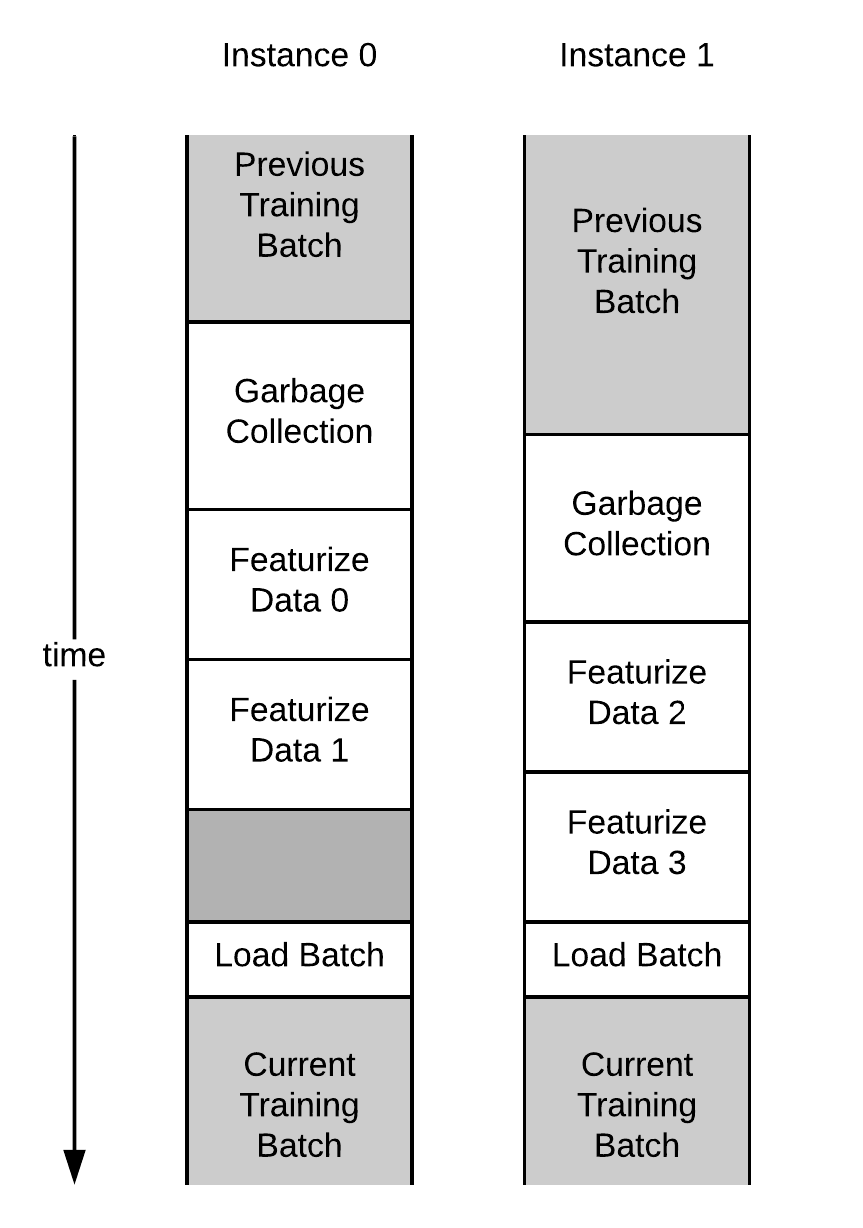
\includegraphics[width=\linewidth]{ci.png}
	\caption{\small 
		Featurization parallelization in the current implementation, with two training instances and batch size of 4. }
	\label{fig:ci}
\end{figure}

In this implementation, each training instance can only write to one exclusive data structure (either MMAP or Manager), which means that we do not need to synchronize all the instances during writing. 
Also, now that the jobs are pre-assigned in a deterministic way, all the instances do not need to communicate with each other before they start performing featurization. 
Hence this implementation alleviates the need for basically all the synchronization. 

However, the caveat comes with this implementation is that, if we have multiple instances with drastically different training speed, the faster ones will always have to wait for the slower ones, since their featurization jobs are distributed evenly, unlike in the original implementation, where the faster instances will be responsible for more featurization jobs. 

During the actual testing, however, we found this disadvantage is ignorable. The reasons are that (1) dataloading consumes about 80\% of the overall training time, which means that the training speed difference between different instances does not matter much at all, and (2) even between models with different network structures, the training speed difference appears to be insignificant. 

\section{Evaluations} \label{sec_eval}

In order to evaluate both implementations in the previous section, we performed a simple test, using about 0.1\% of the fingerprint features trained on fully-connected neural network, on a 4-GPU learning station. 
Note that in order to simulate the CPU training environment, we disabled "feature pre-fetching" option in our models. 

The evaluation results are shown in the table \ref{eval_tb}. 
There are two metrics when it comes to the system performance. 
The first one is training utilization, which is the ratio of actual training time over the total time. 
Higher training utilization means that the system is spending more time on actual training, which indicates its efficiency in dataloading. 
The other metric is the amount of time saved comparing to the vanilla implementation. 
This metric is a more direct indicator for overall system efficiency, and highly correlated to the training utilization. 
However, during the original implementation, we did not have this metric implemented, but the training utilization alone is more than enough as an indicator for the system performance. 

\begin{table*}[!htb]
\centering
\caption{\small Performance Evaluation}
\label{eval_tb}
\resizebox{0.8\linewidth}{!}{%
\begin{tabular}{|l|l|l|l|}
\hline
\multicolumn{2}{|l|}{}                                                                                  & Training Utilization & Time Saved \\ \hline
\multicolumn{2}{|l|}{No Data Sharing}                                                                   & 5.9\%                & -                                    \\ \hline
\multirow{2}{*}{Orignal Implementation} & MMAP (2 Devices)    & 2.2\%                & -                                    \\ \cline{2-4} 
                                                                                  & Manager (2 Devices) & 7.5\%                & -                                    \\ \hline
\multirow{4}{*}{Current Implementation}                                           & MMAP (2 Devices)    & 10.3\%               & 39.4\%                               \\ \cline{2-4} 
                                                                                  & MMAP (4 Devices)    & 14.6\%               & 45.1\%                               \\ \cline{2-4} 
                                                                                  & Manager (2 Devices) & 11.0\%               & 59.6\%                               \\ \cline{2-4} 
                                                                                  & Manager (4 Devices) & 16.8\%               & 66.6\%                               \\ \hline
\end{tabular}}
\end{table*}

In the evaluation results shown in the table \ref{eval_tb}, the current implementation is much more efficient comparing with the original one. 
And the Python Manager data sharing approach appears to perform much better. 
These results align perfectly with the assumptions and analysis we made about the synchronization overhead in the previous chapters. 

Another thing that is worth noticing is that, with more training instances (devices) being used, the training utilization increases significantly. 
This is a clear indication that our implementation scales quite well with the number of training instances. 
We believe that with more concurrent training devices, the system is going to perform even better. 
However, this is yet to be proven during the actual deployment on to the supercomputer. 

In conclusion, our system is shown to save up to 66.6\% time by parallelizing the featurization jobs and sharing features with Python Managers. 
For a single training epoch, our system is estimated to save about 2.3 days of training time, comparing to the no-sharing implementations.

\begin{thebibliography}{}
	\bibitem{ecfp} D. Rogers and M. Hahn, “Extended-Connectivity Fingerprints,” Journal of Chemical Information and Modeling, vol. 50, no. 5, pp. 742–754, 2010.
	\bibitem{lstm} S. Hochreiter and J. Schmidhuber, “Long Short-Term Memory,” Neural Computation, vol. 9, no. 8, pp. 1735–1780, 1997.
	\bibitem{transformer} Vaswani, Ashish, Shazeer, Noam, Parmar, Niki, Jakob, Jones, Gomez, A. N., Kaiser, Lukasz, Polosukhin, and Illia, “Attention Is All You Need,” [astro-ph/0005112] A Determination of the Hubble Constant from Cepheid Distances and a Model of the Local Peculiar Velocity Field, 06-Dec-2017. [Online]. Available: https://arxiv.org/abs/1706.03762. [Accessed: 30-Jan-2019].
	\bibitem{ggnn} Li, Yujia, Tarlow, Daniel, Brockschmidt, Marc, Zemel, and Richard, “Gated Graph Sequence Neural Networks,” [astro-ph/0005112] A Determination of the Hubble Constant from Cepheid Distances and a Model of the Local Peculiar Velocity Field, 22-Sep-2017. [Online]. Available: https://arxiv.org/abs/1511.05493. [Accessed: 30-Jan-2019].
	\bibitem{gcn} T. N. and Max, “Semi-Supervised Classification with Graph Convolutional Networks,” [astro-ph/0005112] A Determination of the Hubble Constant from Cepheid Distances and a Model of the Local Peculiar Velocity Field, 22-Feb-2017. [Online]. Available: https://arxiv.org/abs/1609.02907. [Accessed: 30-Jan-2019].
	\bibitem{gagcn} Ryu, Seongok, Lim, Jaechang, S. Hwan, Kim, and W. Youn, “Deeply learning molecular structure-property relationships using attention- and gate-augmented graph convolutional network,” [astro-ph/0005112] A Determination of the Hubble Constant from Cepheid Distances and a Model of the Local Peculiar Velocity Field, 08-Oct-2018. [Online]. Available: https://arxiv.org/abs/1805.10988. [Accessed: 30-Jan-2019].
	\bibitem{smiles2vec} Goh, G. B., Hodas, N. O., Siegel, Charles, and Abhinav, “SMILES2Vec: An Interpretable General-Purpose Deep Neural Network for Predicting Chemical Properties,” [astro-ph/0005112] A Determination of the Hubble Constant from Cepheid Distances and a Model of the Local Peculiar Velocity Field, 18-Mar-2018. [Online]. Available: https://arxiv.org/abs/1712.02034. [Accessed: 30-Jan-2019].
	\bibitem{chemception} Goh, Garrett, Siegel, Charles, Abhinav, Hodas, N. O., Baker, and Nathan, “Chemception: A Deep Neural Network with Minimal Chemistry Knowledge Matches the Performance of Expert-developed QSAR/QSPR Models,” [astro-ph/0005112] A Determination of the Hubble Constant from Cepheid Distances and a Model of the Local Peculiar Velocity Field, 20-Jun-2017. [Online]. Available: https://arxiv.org/abs/1706.06689. [Accessed: 30-Jan-2019].
	\bibitem{molnet} Wu, Bharath, Feinberg, E. N., Gomes, Joseph, Geniesse, Caleb, Pappu, Karl, and Vijay, “MoleculeNet: A Benchmark for Molecular Machine Learning,” [astro-ph/0005112] A Determination of the Hubble Constant from Cepheid Distances and a Model of the Local Peculiar Velocity Field, 26-Oct-2018. [Online]. Available: https://arxiv.org/abs/1703.00564. [Accessed: 30-Jan-2019].
	\bibitem{gcn_fp} David, Maclaurin, Jorge, Gómez-Bombarelli, Rafael, Hirzel, Alán, Adams, and R. P., “Convolutional Networks on Graphs for Learning Molecular Fingerprints,” [astro-ph/0005112] A Determination of the Hubble Constant from Cepheid Distances and a Model of the Local Peculiar Velocity Field, 03-Nov-2015. [Online]. Available: https://arxiv.org/abs/1509.09292. [Accessed: 30-Jan-2019].
\end{thebibliography}


\end{document}
